\subsection{Cyclopentyl alcohol derivatives}

\subsubsection{Synthesis of the cyclopentyl alcohol head groups }

Synthesis of the cyclopentyl alcohol derivatives began with the synthesis of (1\textit{R},2\textit{R})-2-aminocyclopentan-1-ol \compound{cmpd:HOcy5NH2_RR} and (1\textit{S},2\textit{S})-2-aminocyclopentan-1-ol \compound{cmpd:HOcy5NH2_SS} (see \ref{HOcy5NH2_synth}).
These were synthesised by opening cyclopentene \compound{cmpd:Ocy5} oxide using (\textit{S})-1-phenylethan-1-amine \compound{cmpd:NH2MeBn} to give approximately equal amounts of two diastereomers, \compound{cmpd:HOcy5NHMeBn_RRS} and \compound{cmpd:HOcy5NHMeBn_SSS}, which were separated using column chromatography\cite{Aube1992,Overman1985,Overman1985a}. 
The methylbenzyl group was then removed by hydrogenation to give the two enantiomers of 2-aminocyclopentan-1-ol, \compound{cmpd:HOcy5NH2_RR} and \compound{cmpd:HOcy5NH2_SS}, both in quantitative yield.\todo{this was optimised, maybe add that?}

\begin{scheme}[H]
	\begin{center}
		\schemeref[Ocy5]{cmpd:Ocy5}
		\schemeref[NH2MeBn]{cmpd:NH2MeBn}
		\schemeref[HOcy5NHMeBn_RRS]{cmpd:HOcy5NHMeBn_RRS}
		\schemeref[HOcy5NHMeBn_SSS]{cmpd:HOcy5NHMeBn_SSS}
		\schemeref[HOcy5NH2_RR]{cmpd:HOcy5NH2_RR}
		\schemeref[HOcy5NH2_SS]{cmpd:HOcy5NH2_SS}
		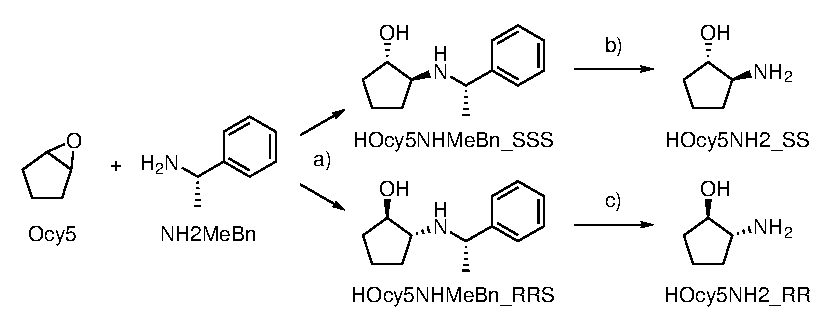
\includegraphics[scale=1]{HOcy5NH2_synth}
		\caption{Synthesis of (1\textit{S},2\textit{S})-2-aminocyclopentan-1-ol \compound{cmpd:HOcy5NH2_SS} and (1\textit{R},2\textit{R})-2-aminocyclopentan-1-ol \compound{cmpd:HOcy5NH2_RR}
		a) \ce{AlMe3}, \ce{CH2Cl2}, 0 $^\circ$C.  \compound{cmpd:HOcy5NHMeBn_SSS} : 35.2 \%,
		\compound{cmpd:HOcy5NHMeBn_RRS} : 32.1 \%.
		b) \ce{Pd(OH)2}, MeOH, \ce{H2}, 5 atm, r.t., 1 d, \compound{cmpd:HOcy5NH2_SS} : 100 \%, \compound{cmpd:HOcy5NH2_RR} : 100 \%.
		\label{sch:HOcy5NH2_synth}}
	\end{center}
\end{scheme}


\renewcommand{\arraystretch}{1.2}
\begin{table}[H]
  \centering
\begin{tabular}{|p{3cm}|c|c|p{3cm}|}
\hline 
Conditions & Temperature/pressure & Time & Result \\ 
\hline 
HCl salt, ammonium formate, 10 \% Pd/C, DMF & r.t. & 2 d & S.M. salt \\ %LMO-2-047
\hline 
Free amine, ammonium formate, 10 \% Pd/C, DMF & r.t. & 2 d & S.M. salt \\ %LMO-2-048
\hline 
HCl salt, ammonium formate, 10 \% Pd/C, dry DMF & r.t. & 2 d & S.M. salt \\ %LMO-2-049
\hline 
Free amine, ammonium formate, 10 \% Pd/C, dry DMF & r.t. & 2 d & S.M. salt \\ %LMO-2-050
\hline 
Free amine, ammonium formate, 10 \% Pd/C, dry DMF & 70 $^{\circ}$C & 1 d & S.M. salt \\ %LMO-2-051
\hline 
Free amine, ammonium formate, 10 \% Pd/C, dry DMF, AcOH & 70 $^{\circ}$C & 1 d & Mess \\ %LMO-2-051
\hline 
HCl salt, dry ammonium formate, 10 \% Pd/C, dry DMF & 120 $^{\circ}$C & 7 d & Unidentified but probably not product \\ %LMO-2-054
\hline 
HCl salt, \ce{Pd(OH)2}, MeOH, H2 & 1 atm & 1 d & S.M. salt \\ %LMO-2-056
\hline 
HCl salt, \ce{Pd(OH)2}, MeOH, H2 & 3.4 atm & 1 d & Possible conversion but lost in work-up \\ %LMO-2-055
\hline 
Free amine, \ce{Pd(OH)2}, MeOH, H2 & 5 atm & 1 d & PRODUCT!!! \\ %LMO-2-057
\hline 
\end{tabular} 
\caption{Conditions attempted for the synthesis ofthe two enantiomers of 2-aminocyclopentan-1-ol, \compound{cmpd:HOcy5NH2_RR} and \compound{cmpd:HOcy5NH2_SS}.\label{tbl:HOcy5NH2_opt}} 
\end{table}

\subsubsection{Initial branching strategy}

An initial retrosynthesis of the conjugates is shown in \ref{sch:HOcy5NH4_retro_A}, and follows a similar path to previous conjugates.

\begin{scheme}[H]
	\begin{center}
		\schemeref[HOcy5NH2_RR]{cmpd:HOcy5NH2_RR}
		\schemeref[HOcy5NH4Br_RR]{cmpd:HOcy5NH4Br_RR}
		\schemeref[HOcy5NH4N3_RR]{cmpd:HOcy5NH4N3_RR}
		\schemeref[HOcy5NH4CipMe_RR]{cmpd:HOcy5NH4CipMe_RR}
		\schemeref[HOcy5NH4T4Cip_RR]{cmpd:HOcy5NH4T4Cip_RR}
		\schemeref[HOcy5NH2_SS]{cmpd:HOcy5NH2_SS}
		\schemeref[HOcy5NH4Br_SS]{cmpd:HOcy5NH4Br_SS}
		\schemeref[HOcy5NH4N3_SS]{cmpd:HOcy5NH4N3_SS}
		\schemeref[HOcy5NH4CipMe_SS]{cmpd:HOcy5NH4CipMe_SS}
		\schemeref[HOcy5NH4T4Cip_SS]{cmpd:HOcy5NH4T4Cip_SS}
		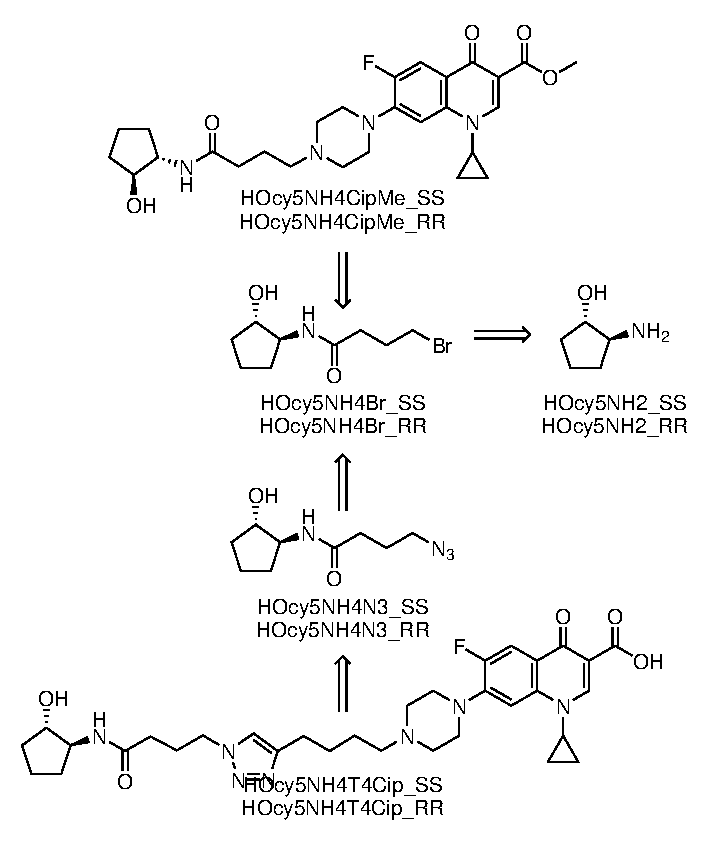
\includegraphics[scale=1]{HOcy5NH4_retro_A_wedges}
		\caption{Retrosynthesis of the cyclopentyl alcohol-CipMe conjugates (\textit{RR}) \compound{cmpd:HOcy5NH4CipMe_RR} and (\textit{SS}) \compound{cmpd:HOcy5NH4CipMe_SS}, and the cyclopentyl alcohol-Cip triazole conjugates (\textit{RR}) \compound{cmpd:HOcy5NH4T4Cip_RR} and (\textit{SS}) \compound{cmpd:HOcy5NH4T4Cip_SS}. \textit{SS} enantiomers are shown, but both will be synthesised. \label{sch:HOcy5NH4_retro_A}}
	\end{center}
\end{scheme}

Synthesis of Br-C$_4$-cyclopentanol-(\textit{SS}) \compound{cmpd:HOcy5NH4Br_SS} from (1\textit{S},2\textit{S})-2-aminocyclopentan-1-ol \compound{cmpd:HOcy5NH2_SS} and 4-bromobutyryl chloride \compound{cmpd:Cl4Br} was attempted using Schotten-Baumann conditions (see \ref{sch:HOcy5NH4Br_SS_synth}). However, a large number of impurities were observed by LCMS (see \ref{fig:HOcy5NH4Br_SS_impurities}), and so three new strategies were attempted: protection of the alcohol (see \ref{sec:TBDMS}), installing the linker on methyl ciprofloxacin \compound{cmpd:CipMe} and then attaching the head group by peptide coupling (see \ref{sec:CipMe_linker}), and using 4-chlorobutyryl chloride \compound{cmpd:Cl4Cl} as the linker instead of 4-bromobutyryl chloride \compound{cmpd:Cl4Br} (see \ref{sec:Cl4Cl}).

%LMO-2-058

\begin{scheme}[H]
	\begin{center}
		\schemeref[HOcy5NH2]{cmpd:HOcy5NH2_SS}
		\schemeref[Cl4Br]{cmpd:Cl4Br}
		\schemeref[HOcy5NH4Br]{cmpd:HOcy5NH4Br_SS}
		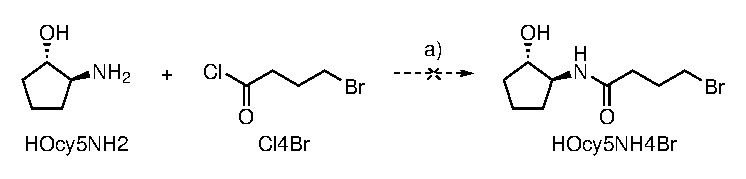
\includegraphics[scale=1]{HOcy5NH4Br_SS_synth}
		\caption{Synthesis of Br-C$_4$-cyclopentanol-(\textit{SS}) \compound{cmpd:HOcy5NH4Br_SS}.
		a) \ce{NaHCO3}, \ce{CH2Cl2}, \ce{H2O}, 0 $^{\circ}$C, 2 h. \label{sch:HOcy5NH4Br_SS_synth}}
	\end{center}
\end{scheme}

\begin{figure}[H]
	\begin{center}
		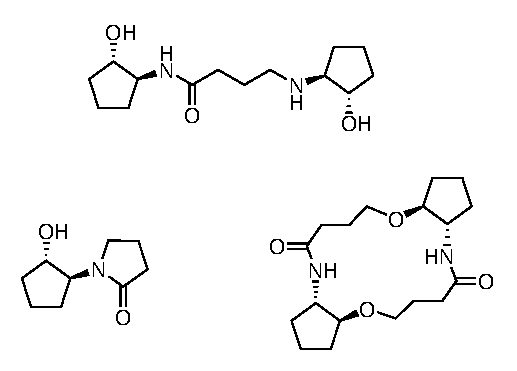
\includegraphics[scale=1]{HOcy5NH4Br_SS_impurities}
		\caption{Impurities observed by LCMS during the synthesis of Br-C$_4$-cyclopentanol-(\textit{SS}) \compound{cmpd:HOcy5NH4Br_SS}.
		Regiochemistry is speculative.
		\label{fig:HOcy5NH4Br_SS_impurities}}
	\end{center}
\end{figure}

\subsubsection{TBDMS protection of the alcohol \label{sec:TBDMS}}

\subsubsubsection{Initial}

The first attempt at an alternative strategy for the synthesis of the conjugates involved TBDMS protection of the alcohol (see \ref{sch:HOcy5NH4_retro_B}). It was envisaged that protection would eliminate enough of the side reactions with products shown in \ref{fig:HOcy5NH4Br_SS_impurities} that intermediates Br-C$_4$-cyclopentanol-(\textit{SS}) \compound{cmpd:HOcy5NH4Br_SS} and N$_3$-C$_4$-cyclopentanol-(\textit{SS}) \compound{cmpd:HOcy5NH4N3_SS} could be purified. The TBDMS group could be removed later in the synthesis using TBAF or acid.

\begin{scheme}[H]
	\begin{center}
		\schemeref[HOcy5NH2_RR]{cmpd:HOcy5NH2_RR}
		\schemeref[TBDMSOcy5NH2_RR]{cmpd:TBSOcy5NH2_RR}
		\schemeref[TBSOcy5NH4Br_RR]{cmpd:TBSOcy5NH4Br_RR}
		\schemeref[TBSOcy5NH4N3_RR]{cmpd:TBSOcy5NH4N3_RR}
		\schemeref[TBSOcy5NH4CipMe_RR]{cmpd:TBSOcy5NH4CipMe_RR}
		\schemeref[TBSOcy5NH4T4Cip_RR]{cmpd:TBSOcy5NH4T4Cip_RR}
		\schemeref[HOcy5NH4CipMe_RR]{cmpd:HOcy5NH4CipMe_RR}
		\schemeref[HOcy5NH4T4Cip_RR]{cmpd:HOcy5NH4T4Cip_RR}
		\schemeref[HOcy5NH2_SS]{cmpd:HOcy5NH2_SS}
		\schemeref[TBSOcy5NH2_SS]{cmpd:TBSOcy5NH2_SS}
		\schemeref[TBSOcy5NH4Br_SS]{cmpd:TBSOcy5NH4Br_SS}
		\schemeref[TBSOcy5NH4N3_SS]{cmpd:TBSOcy5NH4N3_SS}
		\schemeref[TBSOcy5NH4CipMe_SS]{cmpd:TBSOcy5NH4CipMe_SS}
		\schemeref[TBSOcy5NH4T4Cip_SS]{cmpd:TBSOcy5NH4T4Cip_SS}
		\schemeref[HOcy5NH4CipMe_SS]{cmpd:HOcy5NH4CipMe_SS}
		\schemeref[HOcy5NH4T4Cip_SS]{cmpd:HOcy5NH4T4Cip_SS}
		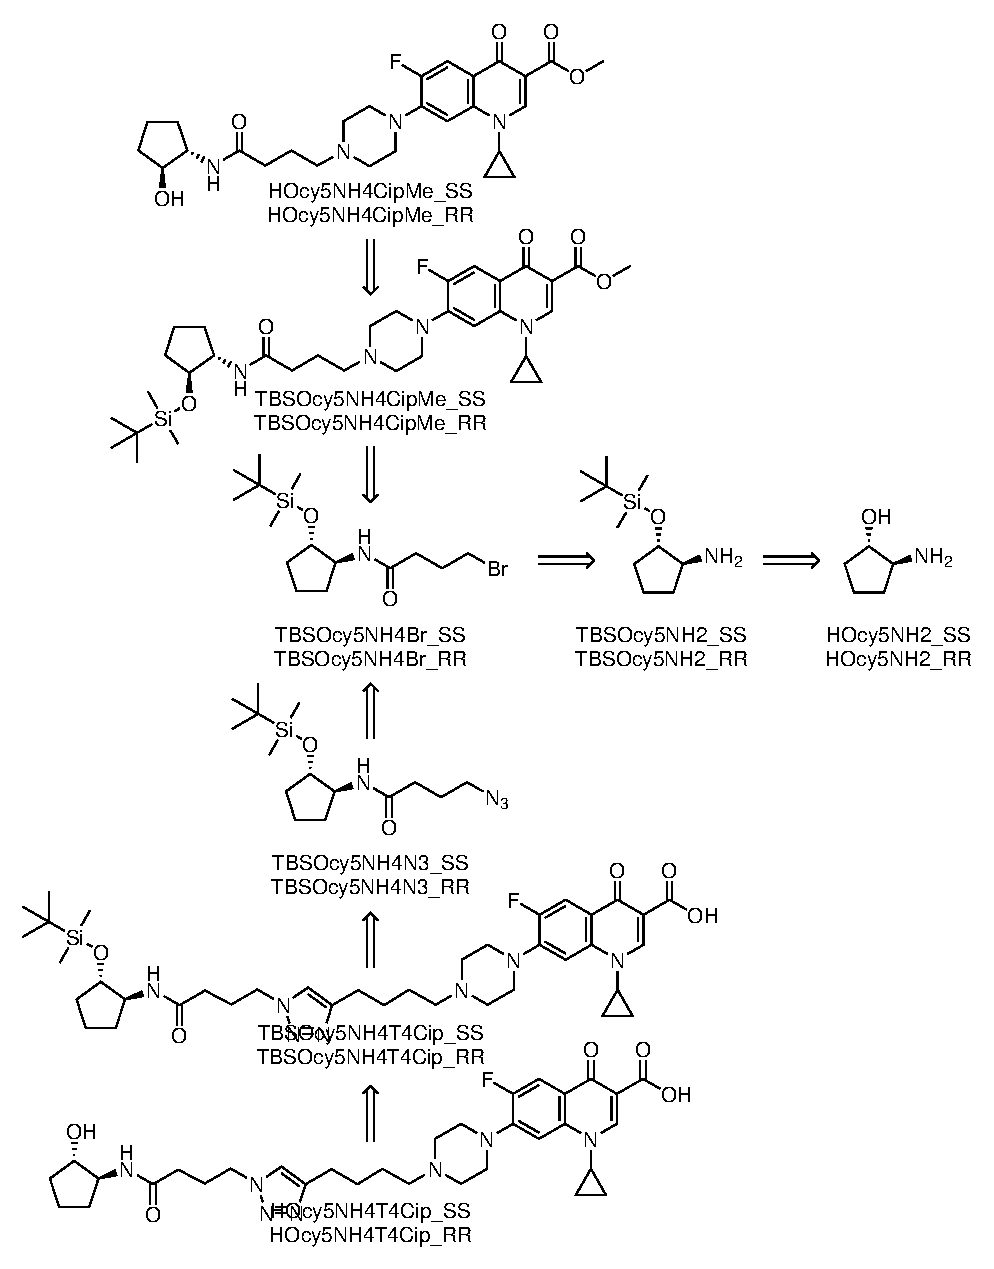
\includegraphics[scale=1]{HOcy5NH4_retro_B}
		\caption{Retrosynthesis of the cyclopentyl alcohol-CipMe conjugates (\textit{RR}) \compound{cmpd:HOcy5NH4CipMe_RR} and (\textit{SS}) \compound{cmpd:HOcy5NH4CipMe_SS}, and the cyclopentyl alcohol-Cip triazole conjugates (\textit{RR}) \compound{cmpd:HOcy5NH4T4Cip_RR} and (\textit{SS}) \compound{cmpd:HOcy5NH4T4Cip_SS} using a TBDMS protection strategy. \textit{SS} enantiomers are shown, but both will be synthesised.\label{sch:HOcy5NH4_retro_B}}
	\end{center}
\end{scheme}

The synthesis began with the optimisation of the protection of (1\textit{S},2\textit{S})-2-aminocyclopentan-1-ol \compound{cmpd:HOcy5NH2_SS} with a TBDMS group on the alcohol. 

\begin{scheme}[H]
	\begin{center}
		\schemeref[HOcy5NH2]{cmpd:HOcy5NH2_SS}
		\schemeref[Cl4Br]{cmpd:Cl4Br}
		\schemeref[TBSOcy5NH2]{cmpd:TBSOcy5NH2_SS}
		\schemeref[TBSOcy5NH4Br]{cmpd:TBSOcy5NH4Br_SS}
		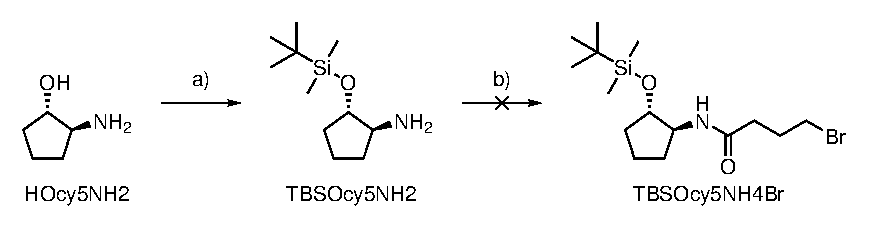
\includegraphics[scale=1]{TBSOcy5NH4Br_SS_synth}
		\caption{The attempted synthesis of Br-C$_4$-cyclopentanol-TBDMS-(\textit{SS}) \compound{cmpd:TBSOcy5NH4Br_SS}. 
		a) See \ref{tbl:TBSOcy5NH4Br_SS_opt}.
		b) \ce{NaHCO3}, \ce{CH2Cl2}, \ce{H2O}, 0 $^{\circ}$C, 2 h. %069,072,073
		\label{sch:TBSOcy5NH4Br_SS_synth}}
	\end{center}
\end{scheme}

\renewcommand{\arraystretch}{1.2}
\begin{table}[H]
  \centering
\begin{tabular}{|p{6cm}|c|c|l|}
\hline 
Conditions & Temperature & Time & Result \\ 
\hline 
TBDMSCl, DMAP, TEA, \ce{CH2Cl2} & r.t. & 18 h & Trace of product? \\ 
\hline 
TBDMSCl, DMAP, TEA, \ce{CH2Cl2} & r.t. & 1 d & Didn't go to completion, lost on prep TLC  \\ 
\hline 
TBDMSCl, imidazole, \ce{CH2Cl2} & 0 $^{\circ}$C & 1 h & S.M. salt in aq layer? \\ 
\hline 
TBDMSCl, DBU, MeCN & 0 $^{\circ}$C & 1 d & S.M. \\ 
\hline 
TBDMSOTf, TEA & 0 $^{\circ}$C & 4 h & Product possibly seen but lost in workup \\ 
\hline 
TBDMSOTf, in 2 portions TEA, \ce{NH4Cl} workup & 0 $^{\circ}$C & 6 h & Product salt? \\ 
\hline 
TBDMSOTf, in 2 portions TEA, aq workup then column & 0 $^{\circ}$C & 6 h & Product! 85 \% \\ 
\hline 
\end{tabular} 
\caption{Conditions attempted for the synthesis of (1\textit{S},2\textit{S})-2-((\textit{tert}-butyldimethylsilyl)oxy)cyclopentan-1-amine \compound{cmpd:TBSOcy5NH2_SS} (see \ref{sch:TBSOcy5NH4Br_SS_synth}).\label{tbl:TBSOcy5NH4Br_SS_opt}} 
\end{table}

Protection optimisation

Still get side-reactions when adding tail

\subsubsubsection{Triazoles by two-step reaction}

Talk about moving to two-step reaction.

\begin{scheme}[H]
	\begin{center}
		\schemeref[TBSOcy5NH2]{cmpd:TBSOcy5NH2_SS}
		\schemeref[Cl4Br]{cmpd:Cl4Br}
		\schemeref[TBSOcy5NH4Br]{cmpd:TBSOcy5NH4Br_SS}		\schemeref[TBSOcy5NH4N3]{cmpd:TBSOcy5NH4N3_SS}
		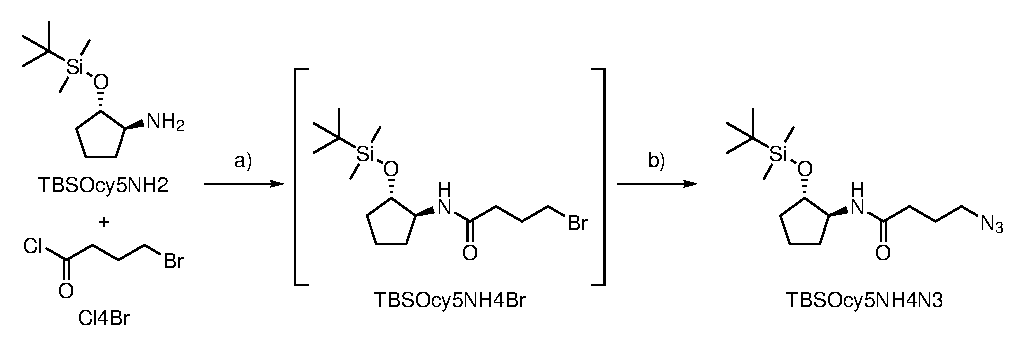
\includegraphics[scale=1]{TBSOcy5NH4N3_SS_synth_2step}
		\caption{
		a) \ce{NaHCO3}, \ce{CH2Cl2}, \ce{H2O}, 0 $^{\circ}$C, 3 h.
		b) \ce{NaN3}, DMF, \ce{CH2Cl2}, r.t., 3 h. 
		99.2 \% over 2 steps. %LMO-2-078
		\label{sch:TBSOcy5NH4N3_SS_synth_2step}}
	\end{center}
\end{scheme}

\begin{scheme}[H]
	\begin{center}
		\schemeref[TBSOcy5NH4N3]{cmpd:TBSOcy5NH4N3_SS}
		\schemeref[Y4Cip]{cmpd:Y4Cip}
		\schemeref[TBSOcy5NH4T4Cip]{cmpd:TBSOcy5NH4T4Cip_SS}
		\schemeref[HOcy5NH4T4Cip]{cmpd:HOcy5NH4T4Cip_SS}
		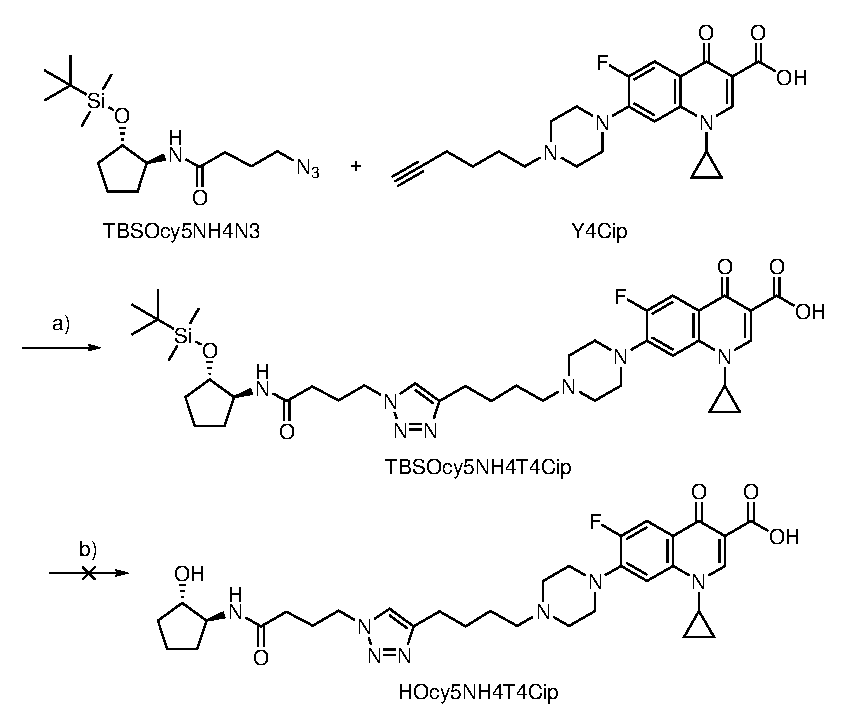
\includegraphics[scale=1]{TBSOcy5NH4T4Cip_SS_synth}
		\caption{
		a) \ce{CuSO4}, sodium ascorbate, THPTA, \ce{H2O}, \textit{t}-BuOH, r.t., 87.4 \%. %, LMO-2-082
		b) TBAF, THF, r.t., 5 d. %LMO-2-084, Lost on purification
		\label{sch:TBSOcy5NH4T4Cip_SS_synth}}
	\end{center}
\end{scheme}

Did click, then failed to deprotect.

\subsubsection{Attaching the linker to ciprofloxacin first\label{sec:CipMe_linker}}

Given the side-reactions and low yields associated with the literate synthesis of the S$_N$2 conjugates proposed by Ganguly et. al\cite{Ganguly2011}, we investigated a second synthesis, building up the linker on the ciprofloxacin side before coupling with the head group (see \ref{sch:HOcy5NH4CipMeRR_synth}).

\begin{scheme}[H]
	\begin{center}
		\schemeref[HOcy5NH2]{cmpd:HOcy5NH2_SS}
		\schemeref[HOO4CipMe]{cmpd:HOO4CipMe}
		\schemeref[tBuOO4CipMe]{cmpd:tBuOO4CipMe}
		\schemeref[tBuOO4Br]{cmpd:tBuOO4Br}
		\schemeref[CipMe]{cmpd:CipMe}
		\schemeref[HOcy5NH4CipMe_SS]{cmpd:HOcy5NH4CipMe_SS}
		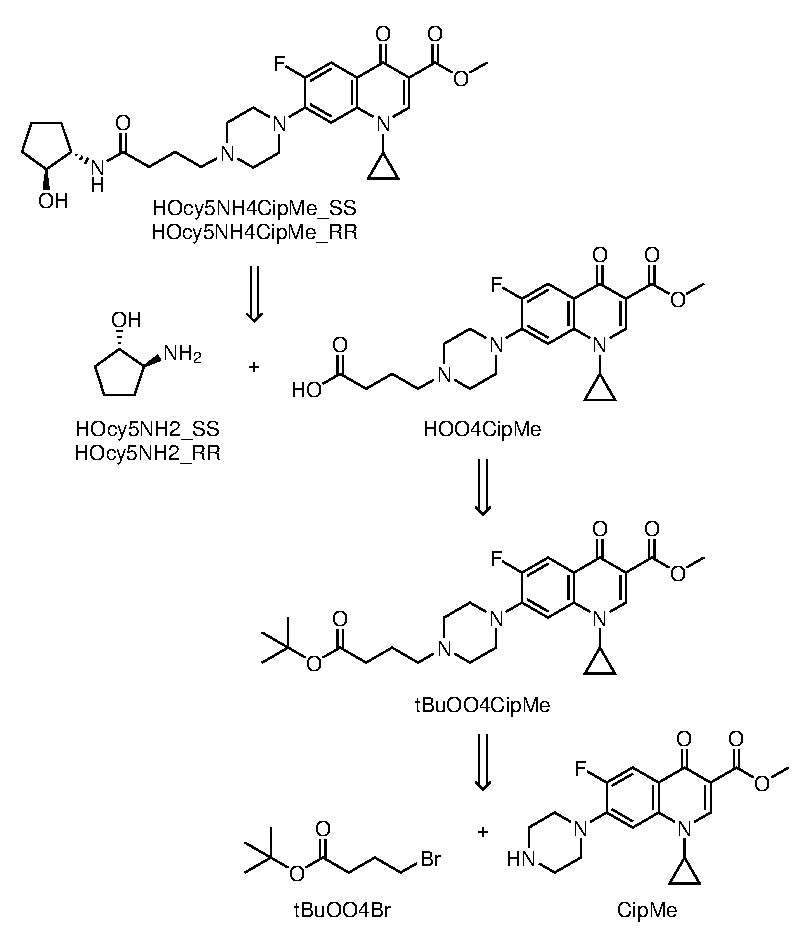
\includegraphics[scale=1]{HOcy5NH4_retro_D}
		\caption{Retrosynthesis of the cyclopentyl alcohol-CipMe conjugates (\textit{RR}) \compound{cmpd:HOcy5NH4CipMe_RR} and (\textit{SS}) \compound{cmpd:HOcy5NH4CipMe_SS}. \textit{SS} enantiomers are shown, but both will be synthesised.\label{sch:HOcy5NH4_retro_D}}
	\end{center}
\end{scheme}

\subsubsubsection{Synthesis of methyl-protected ciprofloxacin with linker with terminal carboxylate}

\begin{scheme}[H]
	\begin{center}
		\schemeref[CipMe]{cmpd:CipMe}
		\schemeref[tBuOO4Br]{cmpd:tBuOO4Br}
		\schemeref[tBuOO4CipMe]{cmpd:tBuOO4CipMe}
		\schemeref[HOO4CipMe]{cmpd:HOO4CipMeTFA}
		\schemeref[HOcy5NH2]{cmpd:HOcy5NH2_SS}
		\schemeref[HOcy5NH4CipMe_SS]{cmpd:HOcy5NH4CipMe_SS}
		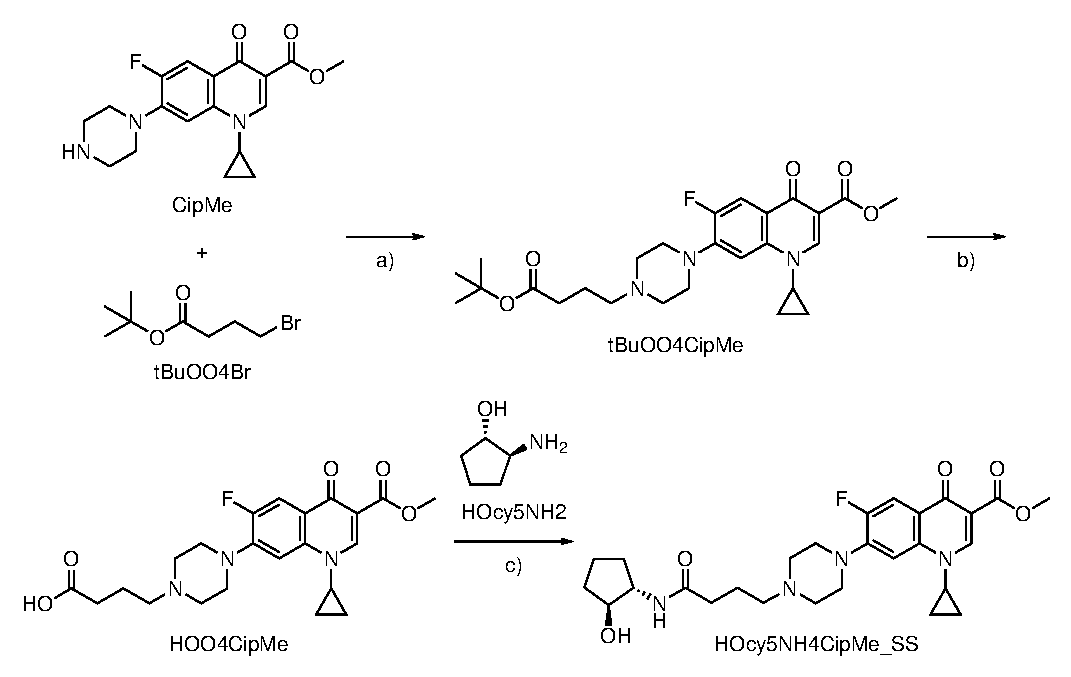
\includegraphics[scale=1]{HOcy5NH4CipMe_SS_synth}
		\caption{Synthesis of \compound{cmpd:HOcy5NH4CipMe_SS}. 
			a) NaI, TEA, MeCN, 100oC, 16h, 50 \%. %, LMO-2-081
			b) TFA,  CH2Cl2, r.t., 18h, 96 \%. %, LMO-2-083. 
			c) EDC, HOBt, DIPEA, DMF, 35 \%. %, LMO-2-093
			\label{sch:HOcy5NH4CipMe_SS_synth}}
	\end{center}
\end{scheme}



\subsubsection{Triazoles from the chloride\label{sec:Cl4Cl}}

\begin{scheme}[H]
	\begin{center}
		\schemeref[HOcy5NH2]{cmpd:HOcy5NH2_SS}
		\schemeref[HOcy5NH4Cl]{cmpd:HOcy5NH4Cl_SS}
		\schemeref[HOcy5NH4N3]{cmpd:HOcy5NH4N3_SS}
		\schemeref[HOcy5NH4CipMe]{cmpd:HOcy5NH4CipMe_SS}
		\schemeref[HOcy5NH4T4Cip]{cmpd:HOcy5NH4T4Cip_SS}
		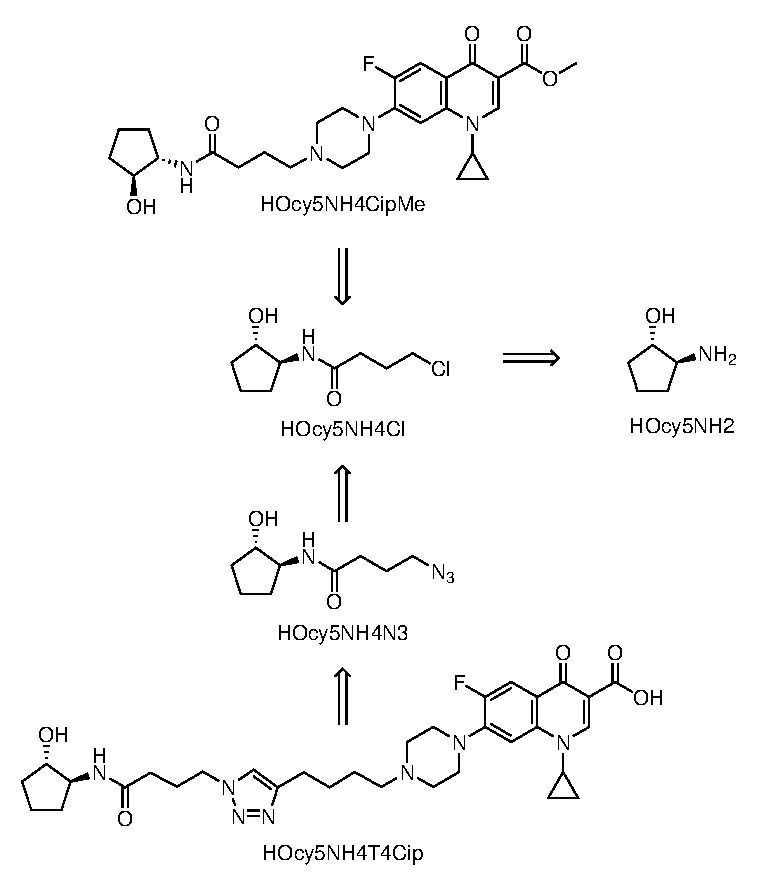
\includegraphics[scale=1]{HOcy5NH4_retro_C}
		\caption{Retrosynthesis of the cyclopentyl alcohol-CipMe conjugates (\textit{RR}) \compound{cmpd:HOcy5NH4CipMe_RR} and (\textit{SS}) \compound{cmpd:HOcy5NH4CipMe_SS}, and the cyclopentyl alcohol-Cip triazole conjugates (\textit{RR}) \compound{cmpd:HOcy5NH4T4Cip_RR} and (\textit{SS}) \compound{cmpd:HOcy5NH4T4Cip_SS} using Cl-C$_4$-cyclopentanol-(\textit{SS}) \compound{cmpd:HOcy5NH4Cl_SS}. \textit{SS} enantiomers are shown, but both will be synthesised.\label{sch:HOcy5NH4_retro_C}}
	\end{center}
\end{scheme}

\begin{scheme}[H]
	\begin{center}
		\schemeref[HOcy5NH2]{cmpd:HOcy5NH2_SS}
		\schemeref[Cl4Cl]{cmpd:Cl4Cl}
		\schemeref[HOcy5NH4Cl]{cmpd:HOcy5NH4Cl_SS}
		\schemeref[HOcy5NH4N3]{cmpd:HOcy5NH4N3_SS}
		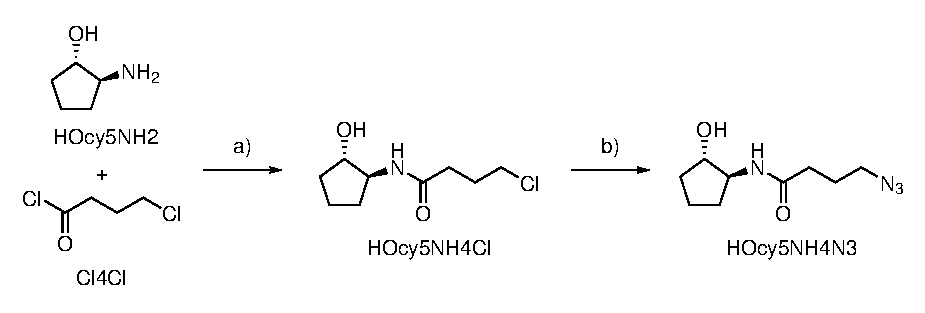
\includegraphics[scale=1]{HOcy5NH4N3_SS_synth}
		\caption{Synthesis of N$_3$-C$_4$-cyclopentanol-(\textit{SS}) \compound{cmpd:HOcy5NH4N3_SS}.
		a) TEA, \ce{CH2Cl2}, 0 $^{\circ}$C, 2 h.
		b) \ce{NaN3}, acetonitrile, 50 $^\circ$C, 24 h, 45.0 \%. \label{sch:HOcy5NH4N3_SS_synth}}
	\end{center}
\end{scheme}

\begin{scheme}[H]
	\begin{center}
		\schemeref[HOcy5NH4N3]{cmpd:HOcy5NH4N3_SS}
		\schemeref[Y4Cip]{cmpd:Y4Cip}
		\schemeref[HOcy5NH4T4Cip]{cmpd:HOcy5NH4T4Cip_SS}
		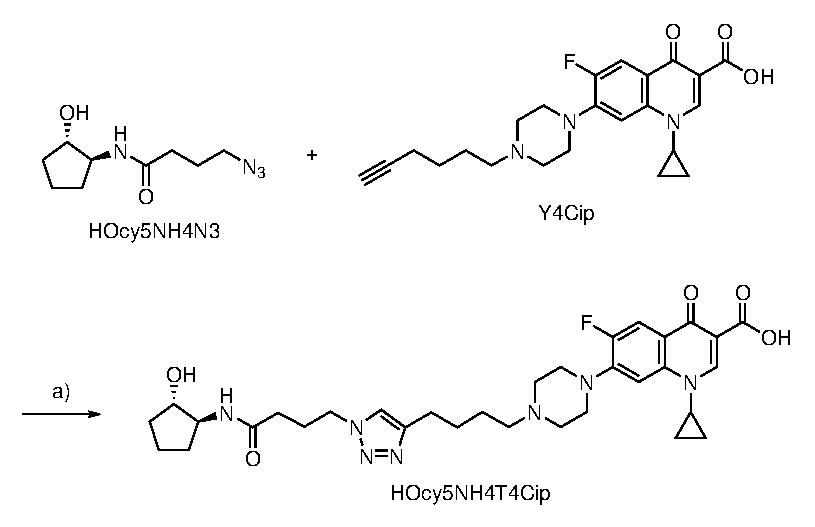
\includegraphics[scale=1]{HOcy5NH4T4Cip_RR_synth}
		\caption{Synthesis of the cyclopentyl alcohol-Cip triazole conjugate \compound{cmpd:HOcy5NH4T4Cip_SS}. 
		a) \ce{CuSO4}, THPTA, sodium ascorbate, \ce{H2O}, \textit{t}-BuOH, \ce{CH2Cl2}, r.t., 3 d, 22.2 \%.\label{sch:HOcy5NH4T4Cip_RR_synth}}
	\end{center}
\end{scheme}

This worked.
